\newcommand{\prob}{\rho}

\documentclass[tikz]{standalone}
\usepackage{comment}
\usetikzlibrary{arrows,shapes,automata,petri,positioning,calc}
\usepackage{xcolor}
\definecolor{darkblue}{rgb}{0.2,0.2,0.6}
\definecolor{darkred}{rgb}{0.6,0.1,0.1}
\definecolor{darkgreen}{rgb}{0.2,0.6,0.2}

\definecolor{acsiorange}{RGB}{180,88,26}
\definecolor{acsired}{RGB}{150,0,0}
\definecolor{acsigreen}{RGB}{128,198,54}
\definecolor{acsiblue}{RGB}{43,80,150}

%%%%%%%%%%%%%%%%%%%%%%%%%%%%%%%%%%%%%%%%
\definecolor{swimmyred}{RGB}{206,19,55}
\definecolor{marcofucsia1}{RGB}{203,41,123}
\definecolor{marcofucsia1}{RGB}{203,41,123}
\definecolor{marcofucsia2}{RGB}{153,25,94}
\definecolor{marcofucsia3}{RGB}{102,29,70}
\definecolor{marcoblue1}{RGB}{17,183,225}
\definecolor{marcoblue2}{RGB}{16,163,201}
\definecolor{marcoblue3}{RGB}{5,132,165}
\definecolor{marcoblue4}{RGB}{4,105,131}
\definecolor{marcoblue5}{RGB}{0,77,128}
\definecolor{marcoorange}{RGB}{255,147,0}
\definecolor{marcogreen1}{RGB}{82,174,139}
\definecolor{marcogreen2}{RGB}{56,122,101}


\newcommand{\tcolor}{\color{marcofucsia3}}
\newcommand{\wcolor}{\color{marcofucsia1}}
\newcommand{\pcolor}{\color{violet}}

%%%%%%%%%%%%%%%%%%% PETRI %%%%%%%%%%%%%%%%%%%%%%%%
\usetikzlibrary{arrows,shapes,automata,petri,positioning,calc}

\tikzset{
	place/.style={
		circle,
		very thick,
		draw=acsiblue!90,
		fill=acsiblue!10,
		minimum size=6mm,
	},
    tasktrans/.style={
        transition,
		rectangle,
		very thick,
		fill=marcofucsia3!10,
        draw=marcofucsia3!100,
		minimum width=5mm,
        minimum height=5mm,
		inner ysep=2pt
	},
	transitionH/.style={
		rectangle,
		thick,
		fill=black,
		minimum width=6mm,
		inner ysep=2pt
	},
	transitionV/.style={
		rectangle,
		thick,
		fill=black,
		minimum height=6mm,
		inner xsep=2pt
	},
    tautrans/.style={
      tasktrans,
      fill=black!100,
      draw=black!100,
      font=\color{white},
    },
    arc/.style={
        -angle 90,
        thick,
    },
	state/.style={
		rectangle,
        rounded corners=5pt,
        draw,
		very thick,
		fill=orange!10,
		minimum height=5mm,
		minimum width=10mm,
	},
    link/.style={
        -stealth,
        thick,
    },
	config/.style={
		circle,
        rounded corners=5pt,
        draw,
		very thick,
        fill=black,
		minimum height=2mm,
		minimum width=2mm,
        font=\tiny\color{white}
	},
    hconfig/.style={
		circle,
        rounded corners=5pt,
     	minimum height=2mm,
		minimum width=2mm,
        font=\tiny\color{white}
	},
}



\tikzstyle{joint}=[
 	circle,
	minimum size=1mm,
    draw,
    very thick,
]

\tikzstyle{cjoint}=[
    joint,
    fill=marcoorange!80,
]

\tikzstyle{pjoint}=[
    joint,
    fill=marcoorange!30,
]

\tikzstyle{cstep}=[
    rectangle,
    rounded corners=5pt,
    minimum height=3.5em,
    minimum width=5em,
    very thick,
    draw,
    fill=marcoblue1!40,
    font=\footnotesize
]

\tikzstyle{astep}=[
    rectangle,
    minimum height=4.2em,
    minimum width=5em,
    thick,
    draw,
    fill=marcoblue2!20,
    inner sep=5,
]

\tikzset{database/.style={cylinder,aspect=0.5,draw,rotate=90,path picture={
			\draw (path picture bounding box.160) to[out=180,in=180] (path picture bounding
			box.20);
			\draw (path picture bounding box.200) to[out=180,in=180] (path picture bounding
			box.340);
}}}





\begin{document}

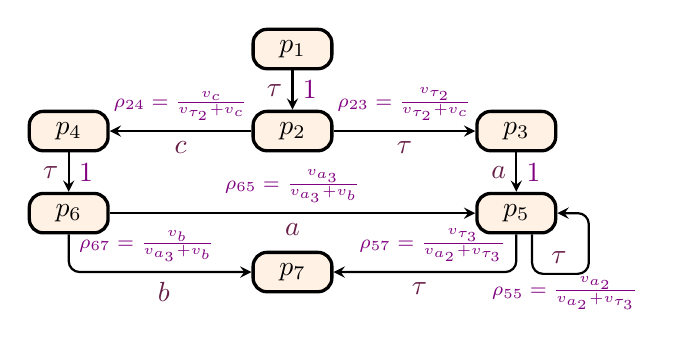
\begin{tikzpicture}[node distance=0.5cm and 1.8cm,>=stealth',bend angle=45,auto]
	
\node[state] (i) {$p_1$};
\node[state] (ii) [below=of i] {$p_2$};
\node[state] (iii) [right=of ii] {$p_3$};
\node[state] (iv) [left=of ii] {$p_4$};
\node[state] (v) [below=of iii] {$p_5$};
\node[state] (vi) [below=of iv] {$p_6$};
\node[below=of ii] (dot) {};
\node[state] (vii) [below=of dot] {$p_7$};

\draw[link] 
  (i) 
  -- 
  node[right]{\pcolor $1$} 
  node[left]{\tcolor $\tau$}
  (ii);

\draw[link] 
  (ii) 
  -- 
  node[above,font=\scriptsize]{\pcolor $\prob_{23} = \frac{v_{\tau_2}}{v_{\tau_2}+v_c}$} 
  node[below]{\tcolor $\tau$}
  (iii);

\draw[link] 
  (ii) 
  -- 
  node[above,font=\scriptsize]{\pcolor $\prob_{24} = \frac{v_c}{v_{\tau_2}+v_c}$} 
  node[below]{\tcolor $c$}
  (iv);
\draw[link] 
  (iii) 
  -- 
  node[right]{\pcolor $1$} 
  node[left]{\tcolor $a$}
  (v);

\draw[link] 
  (iv) 
  -- 
  node[right]{\pcolor $1$} 
  node[left]{\tcolor $\tau$}
  (vi);


\draw[link,rounded corners=4pt,] 
  (v) 
  |-
  node[above left,font=\scriptsize]{\pcolor $\prob_{57} = \frac{v_{\tau_3}}{v_{a_2}+v_{\tau_3}}$} 
  node[below left,xshift=-10mm]{\tcolor $\tau$}
  (vii);

\draw[link,rounded corners=4pt] 
  ($(v.south)+(2mm,0)$) 
  |-
  ($(v.south east)+(4mm,-5mm)$)  
  node[below,font=\scriptsize,yshift=1mm,xshift=-3mm]{\pcolor $\prob_{55} = \frac{v_{a_2}}{v_{a_2}+v_{\tau_3}}$} 
  node[above left,xshift=-1.5mm]{\tcolor $\tau$}
  |-
  (v.east);


\draw[link] 
  (vi) 
  -- 
  node[above,font=\scriptsize]{\pcolor $\prob_{65} = \frac{v_{a_3}}{v_{a_3}+v_b}$} 
  node[below]{\tcolor $a$}
  (v);

\draw[link,rounded corners=4pt,] 
  (vi) 
  |-
  node[above right,font=\scriptsize]{\pcolor $\prob_{67} = \frac{v_{b}}{v_{a_3}+v_b}$} 
  node[below right,xshift=10mm]{\tcolor $b$}
  (vii);

\end{tikzpicture}
	
\end{document}